The galapagos architecture is MIMD architecture with shared memory. This imposes problems when more fitness cores need to access the memory simultaneously. In order to overcome this problem the access to the memory is controlled with a memory controller. The responsibility of the memory controller is granting access and performing memory related tasks on behalf of the requesting fitness cores. The controller is constructed in a way that only allows one fitness core to be able to carry out a memory request at a single time. In case of multiple memory requests, the controller performs a selection deciding in which order the requesting cores is granted the bus. The precise technique of selection can be seen in algorithm \ref{algorithm:round-robin-selection}

\begin{figure}[H]
\begin{algorithm}[H]
\SetAlgoLined
\DontPrintSemicolon
\KwData{Requests - requests signals from the fitness cores\newline 
Request - 2-bits specifying the operation}
\Begin{
    $ Requests \longleftarrow $ requests from the fitness cores\;
    \While{$ True $}{
        \For {Request in Requests} {
        \uIf{request $=$ asserted}{
            performMemoryOperation()
        }
         \Else{
        continue
        }           
        }
        
    }
}
\caption{Round-robin selection}
\label{algorithm:round-robin-selection}
\end{algorithm}
\end{figure}


These algorithm is based on round-robin scheduling. The request bits of \emph{fitness cores} are checked in turn to check if one of the cores has requested the memory bus. The type of request is determined by combination of two request signals sent by each \emph{fitness core}. The signals refer to either a \emph{NOP}, \emph{READ}, or \emph{WRITE} operation. In case of \emph{NOP} the algorithms move to check the next state request lines. It moves in this fashion until a \emph{READ} or \emph{WRITE} request is encountered. 

When a \emph{READ} or \emph{WRITE} operation is encountered, the \emph{data controller} starts to carry out the request from the fitness core. Note that the the memory buses from and to the memory are 16-bits wide. This implies that  it requires at least for cycles in order to transmit/receive 64-bits data over the buses. In addition, external memory requires different control signals. These control signals need to be asserted or de-asserted at specific times when performing the operation. The timing diagrams for the memory chip can be seen in figure (?) \todo{Add timing diagram for memory chip}

This requires the memory controller to use the specific communication protocol when transmitting/receiving data from memory. To accomplish this communication, the memory controller is implemented as a state machine. The responsibility of the state machine is to divide the functionality required to write and read into different cycles. \todo{More details required} \todo{Add reference}



\begin{figure}

  \centering
  % Trim er [left bottom right top]
  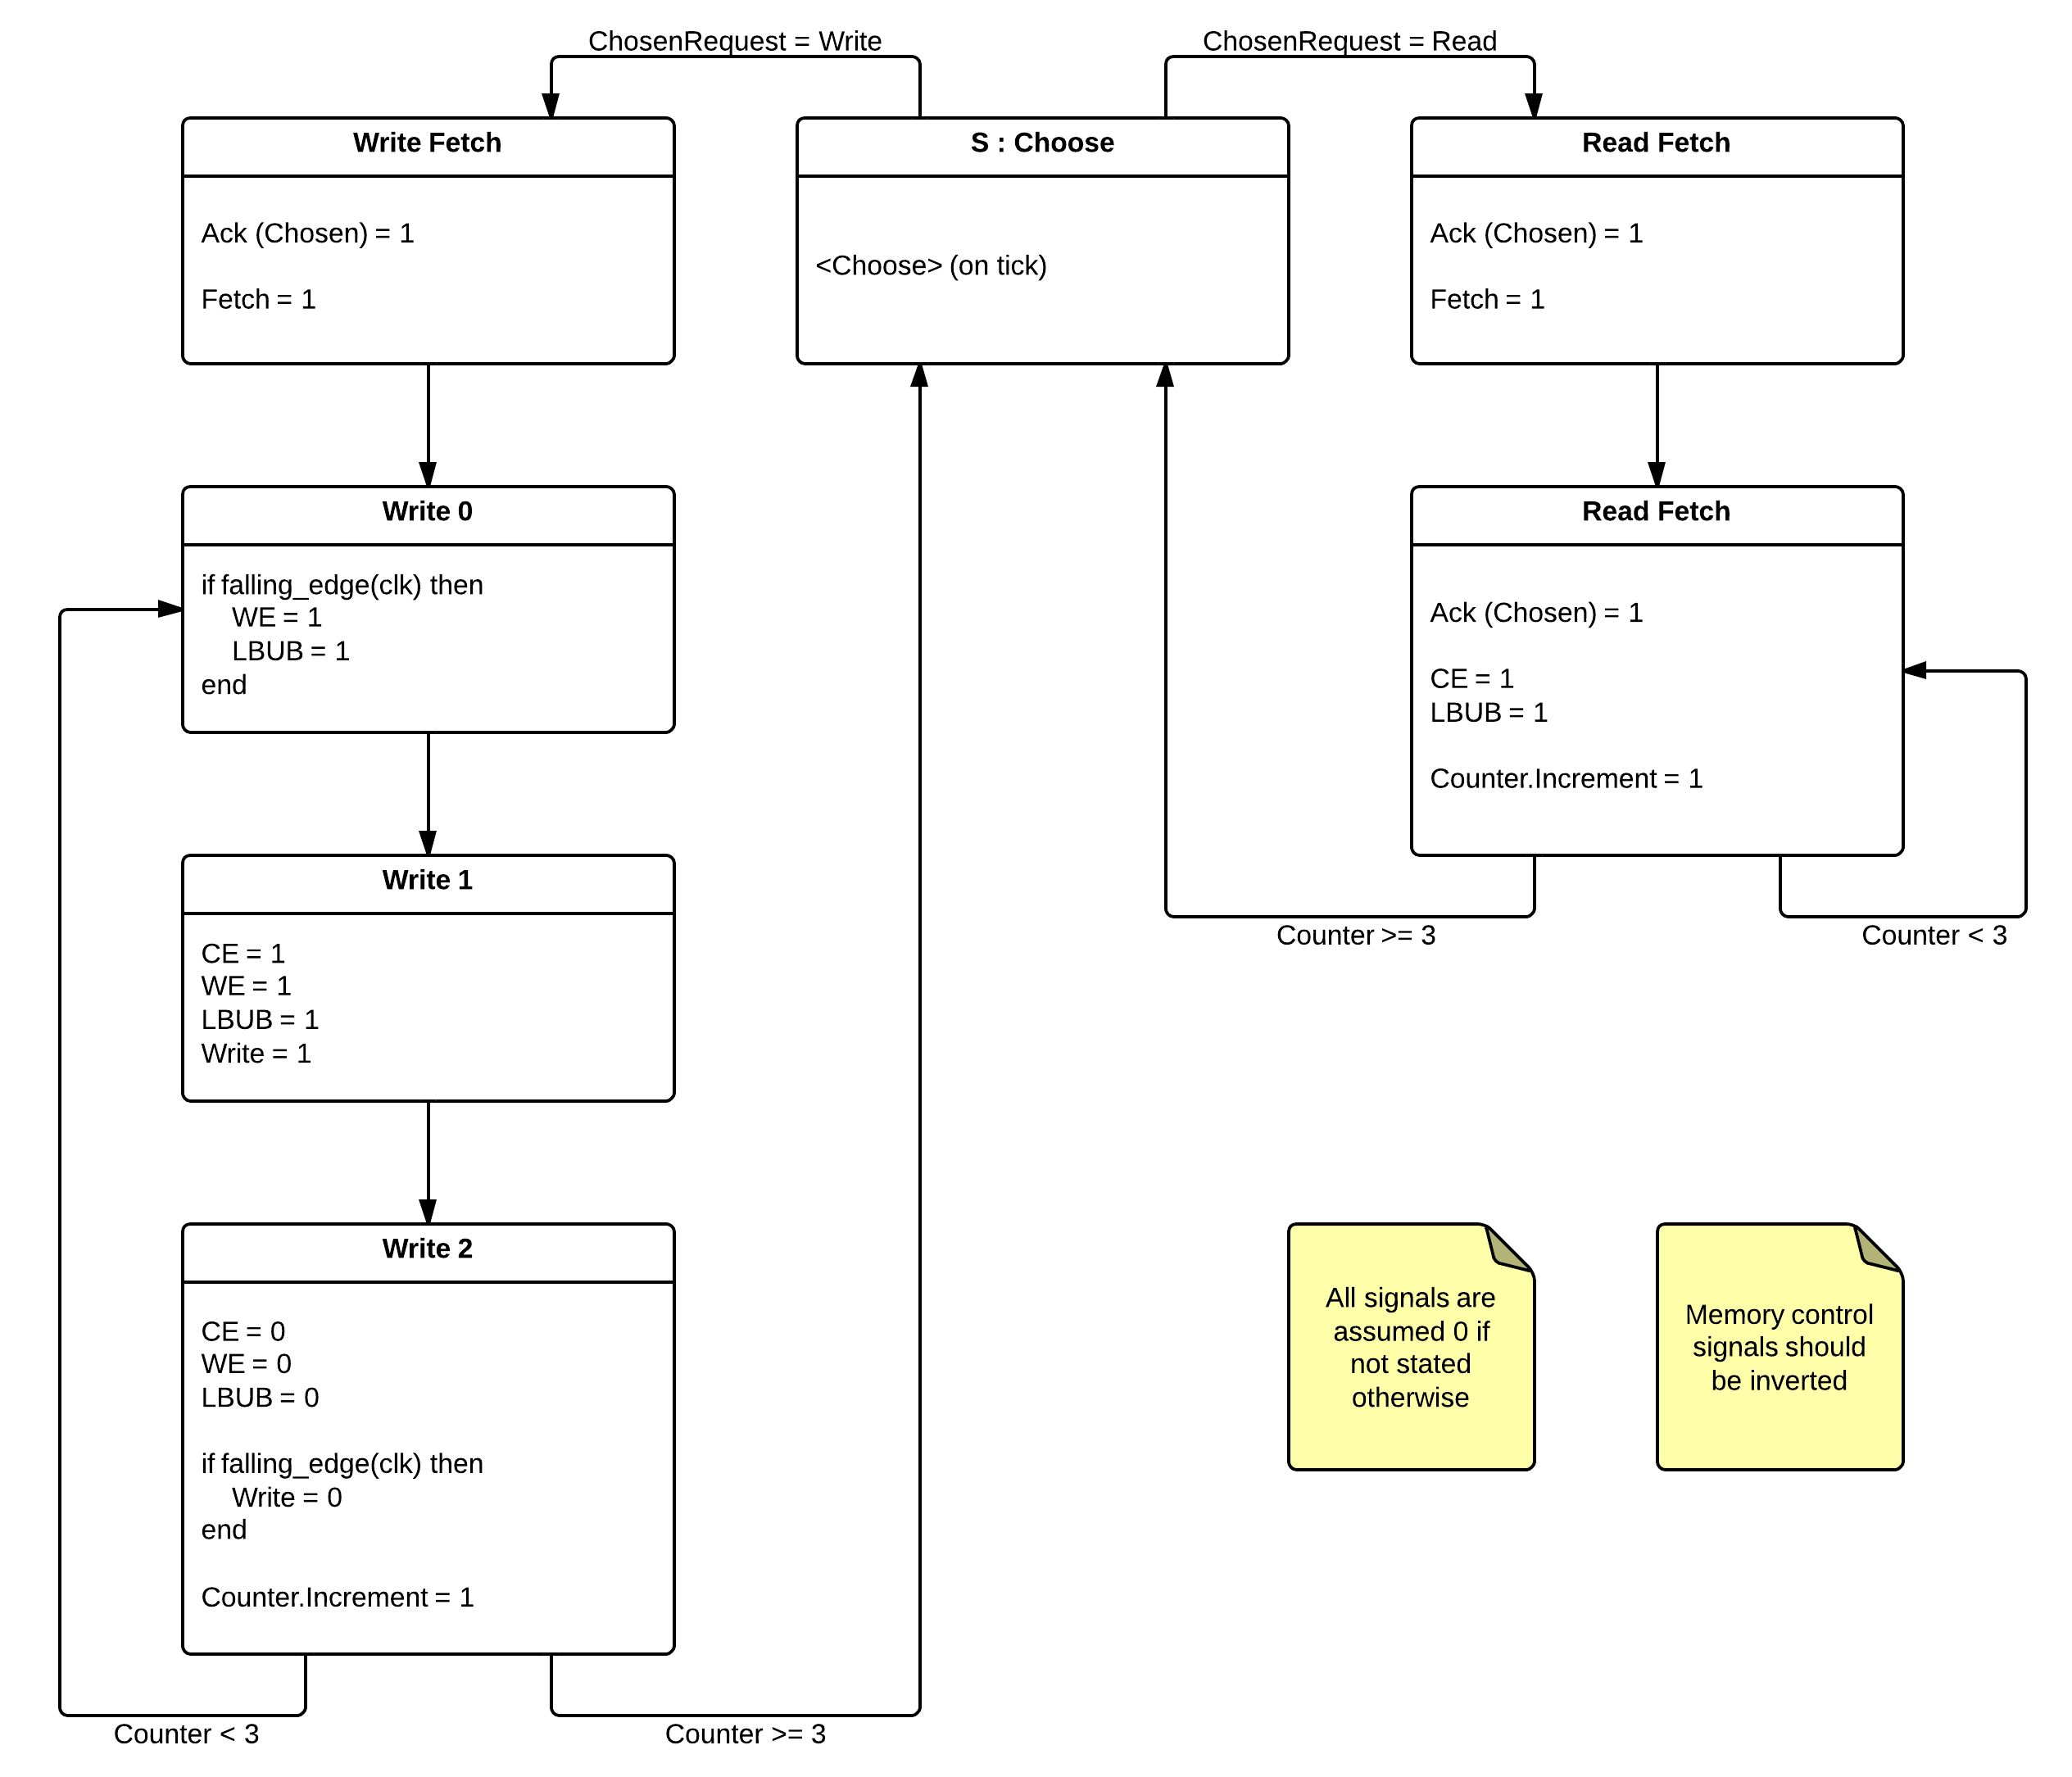
\includegraphics[width=\textwidth]{fpga/fig/memory_ctrl_state_machine.png}
  \caption{Data memory controller state machine}
  \label{fpga:fig:mem:data_memory_ctrl}
\end{figure}



 








